\section{Auswertung der OPC Factory Plattform}
\label{sec:OPCFactory}

Während eines Informatik-Bachelorpraktikums „Mojito, Caipirinha, Sex on the Beach – Die Rezepte des BAR-Robots müssen auf eine Plattform“ wurde bereits 2019 die „OPC Factory“ Platform entwickelt, dessen Anwendungsfall dem in dieser Arbeit präsentierten nicht unähnlich ist [\cite{bp}]. In Grafik \ref{fig:OPCFactoryBenutzeroberfläche} ist die Benutzeroberfläche dieser Anwendung abgebildet.
%
\begin{figure}[htbp]
	\centering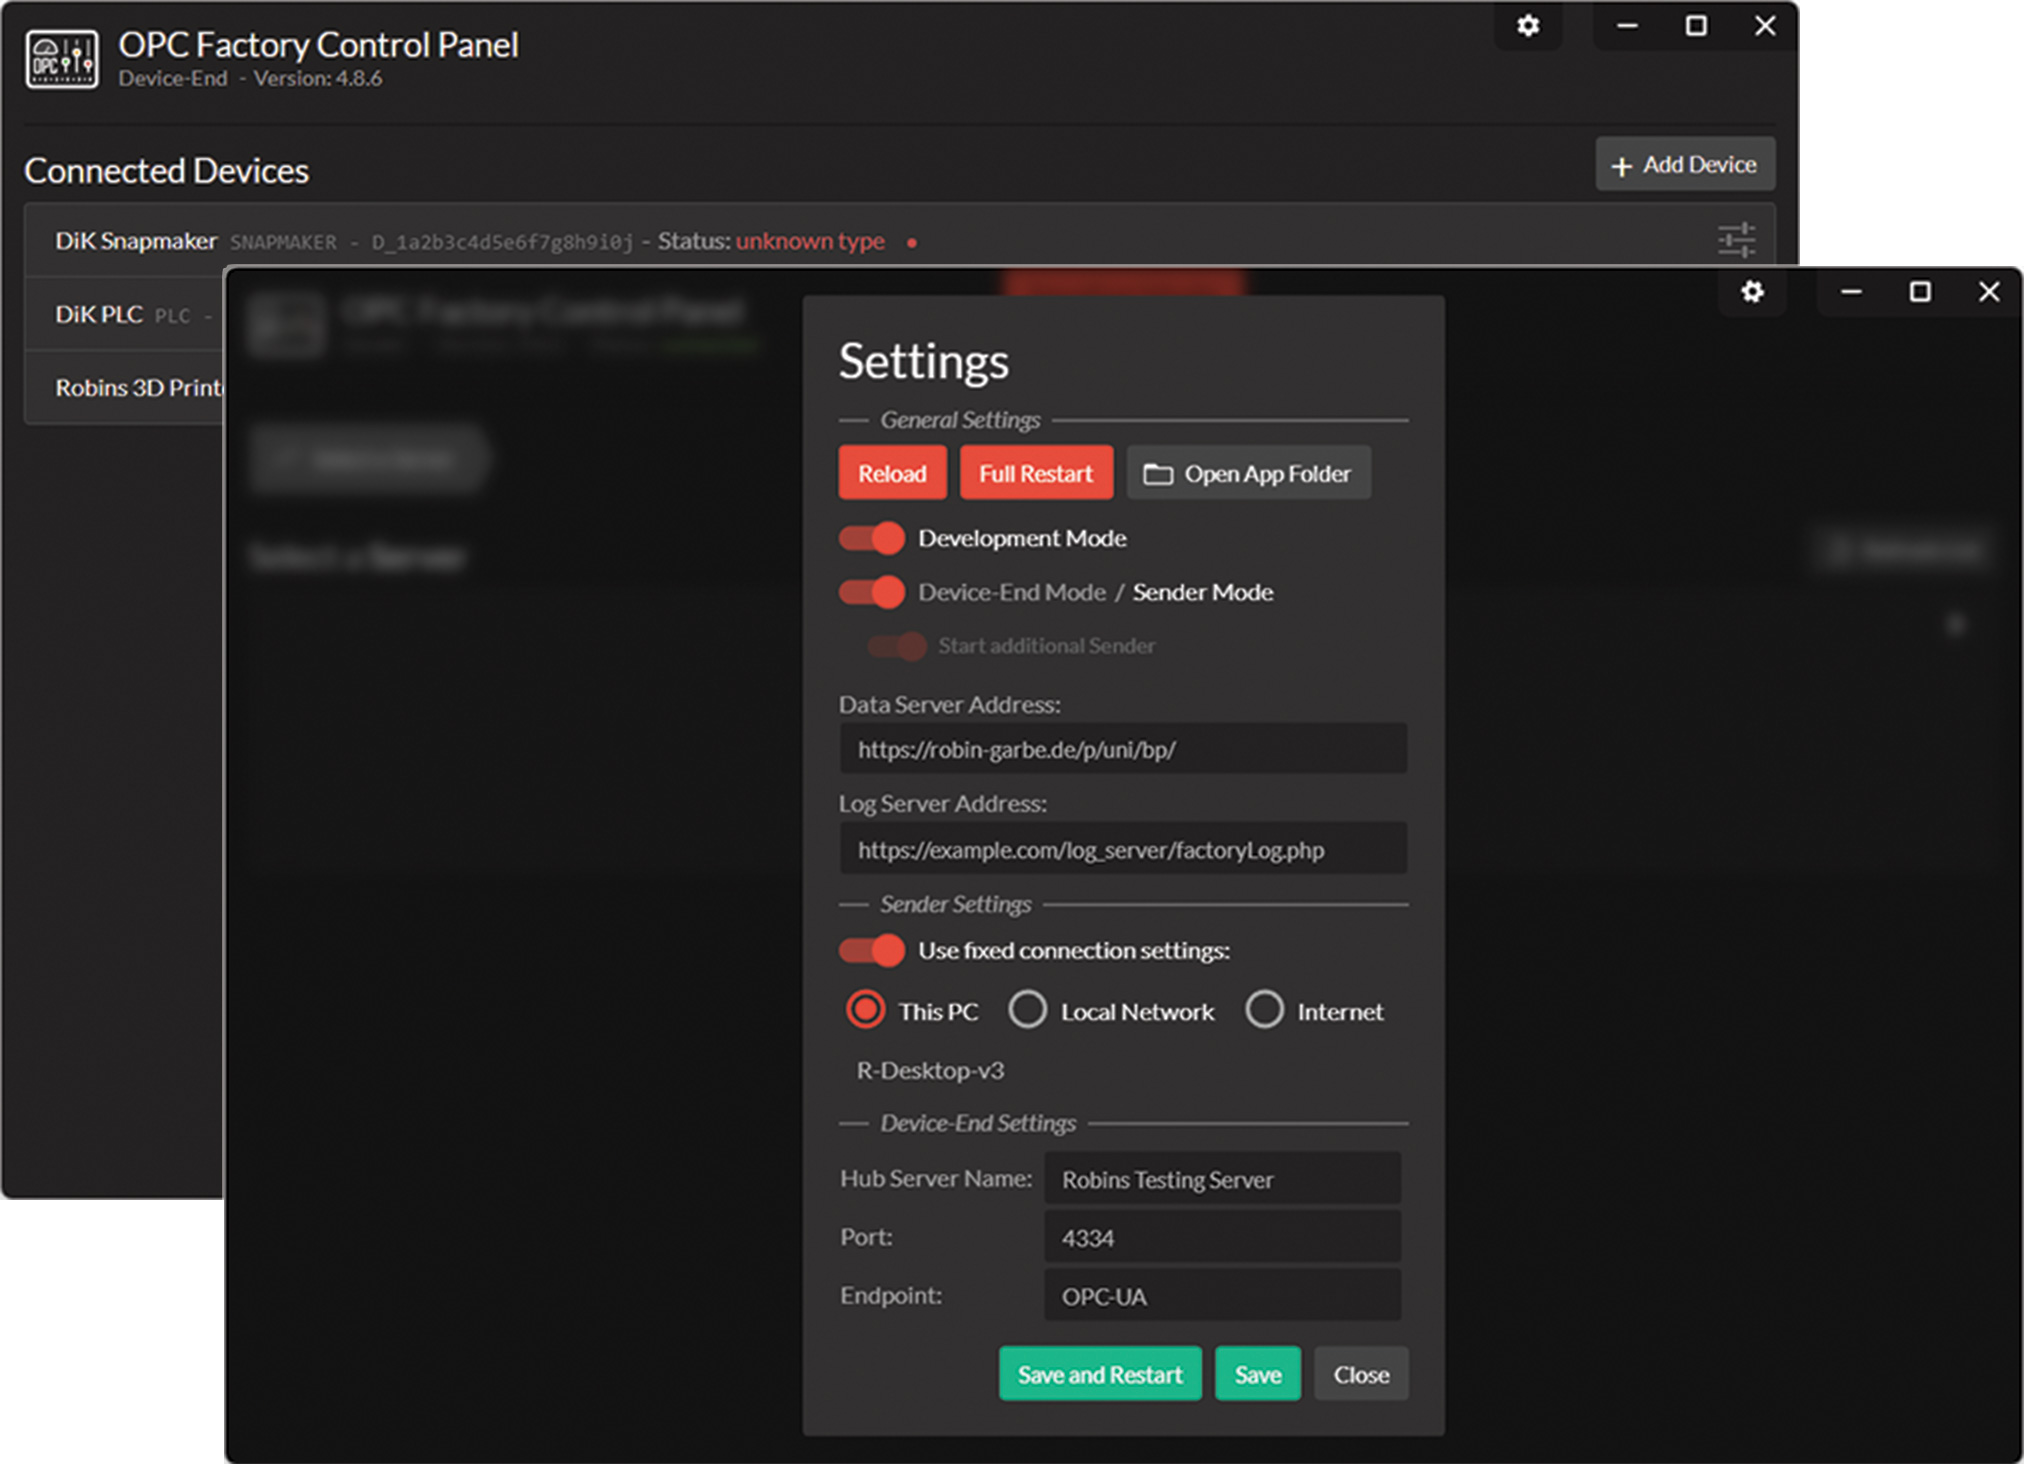
\includegraphics[width=1.0\textwidth]{images/04/OPC_Factory.jpg}
    \caption{Benutzeroberfläche der OPC Factory}
    \label{fig:OPCFactoryBenutzeroberfläche}
\end{figure}

Die OPC Factory ist zusammenfassend ausgedrückt eine Applikation, welche aus einem Server („Device-End“) und einem Client („Sender“) besteht, und welche genutzt werden kann, um auf einer Vielzahl von verbundenen Maschinen vordefinierte Aufträge auszuführen. Das System was dabei serviceorientiert und flexibel gestaltet, sodass ein Server sich mit beliebig vielen Endgeräten verbinden kann und ein Client alle Endgeräten von beliebig vielen Servern ansprechen kann. Eine Besonderheit ist hier, dass die Verbindung zu den Endgeräten modular gestaltet ist. Das heißt, dass ursprünglich PLCs über OPC-UA sowie über USB verbundene Geräte mittels einer seriellen Verbindung angesprochen werden konnten, dies jedoch um beliebige weitere Gerätetypen erweitert werden kann. Die Kommunikations-Infrastruktur der OPC Factory ist in Grafik \ref{fig:OPCFactoryInfrastruktur} abgebildet. Der Datenaustausch zwischen dem Client und dem Server läuft in dieser Applikation mittels OPC-UA.
%
\begin{figure}[htbp]
	\centering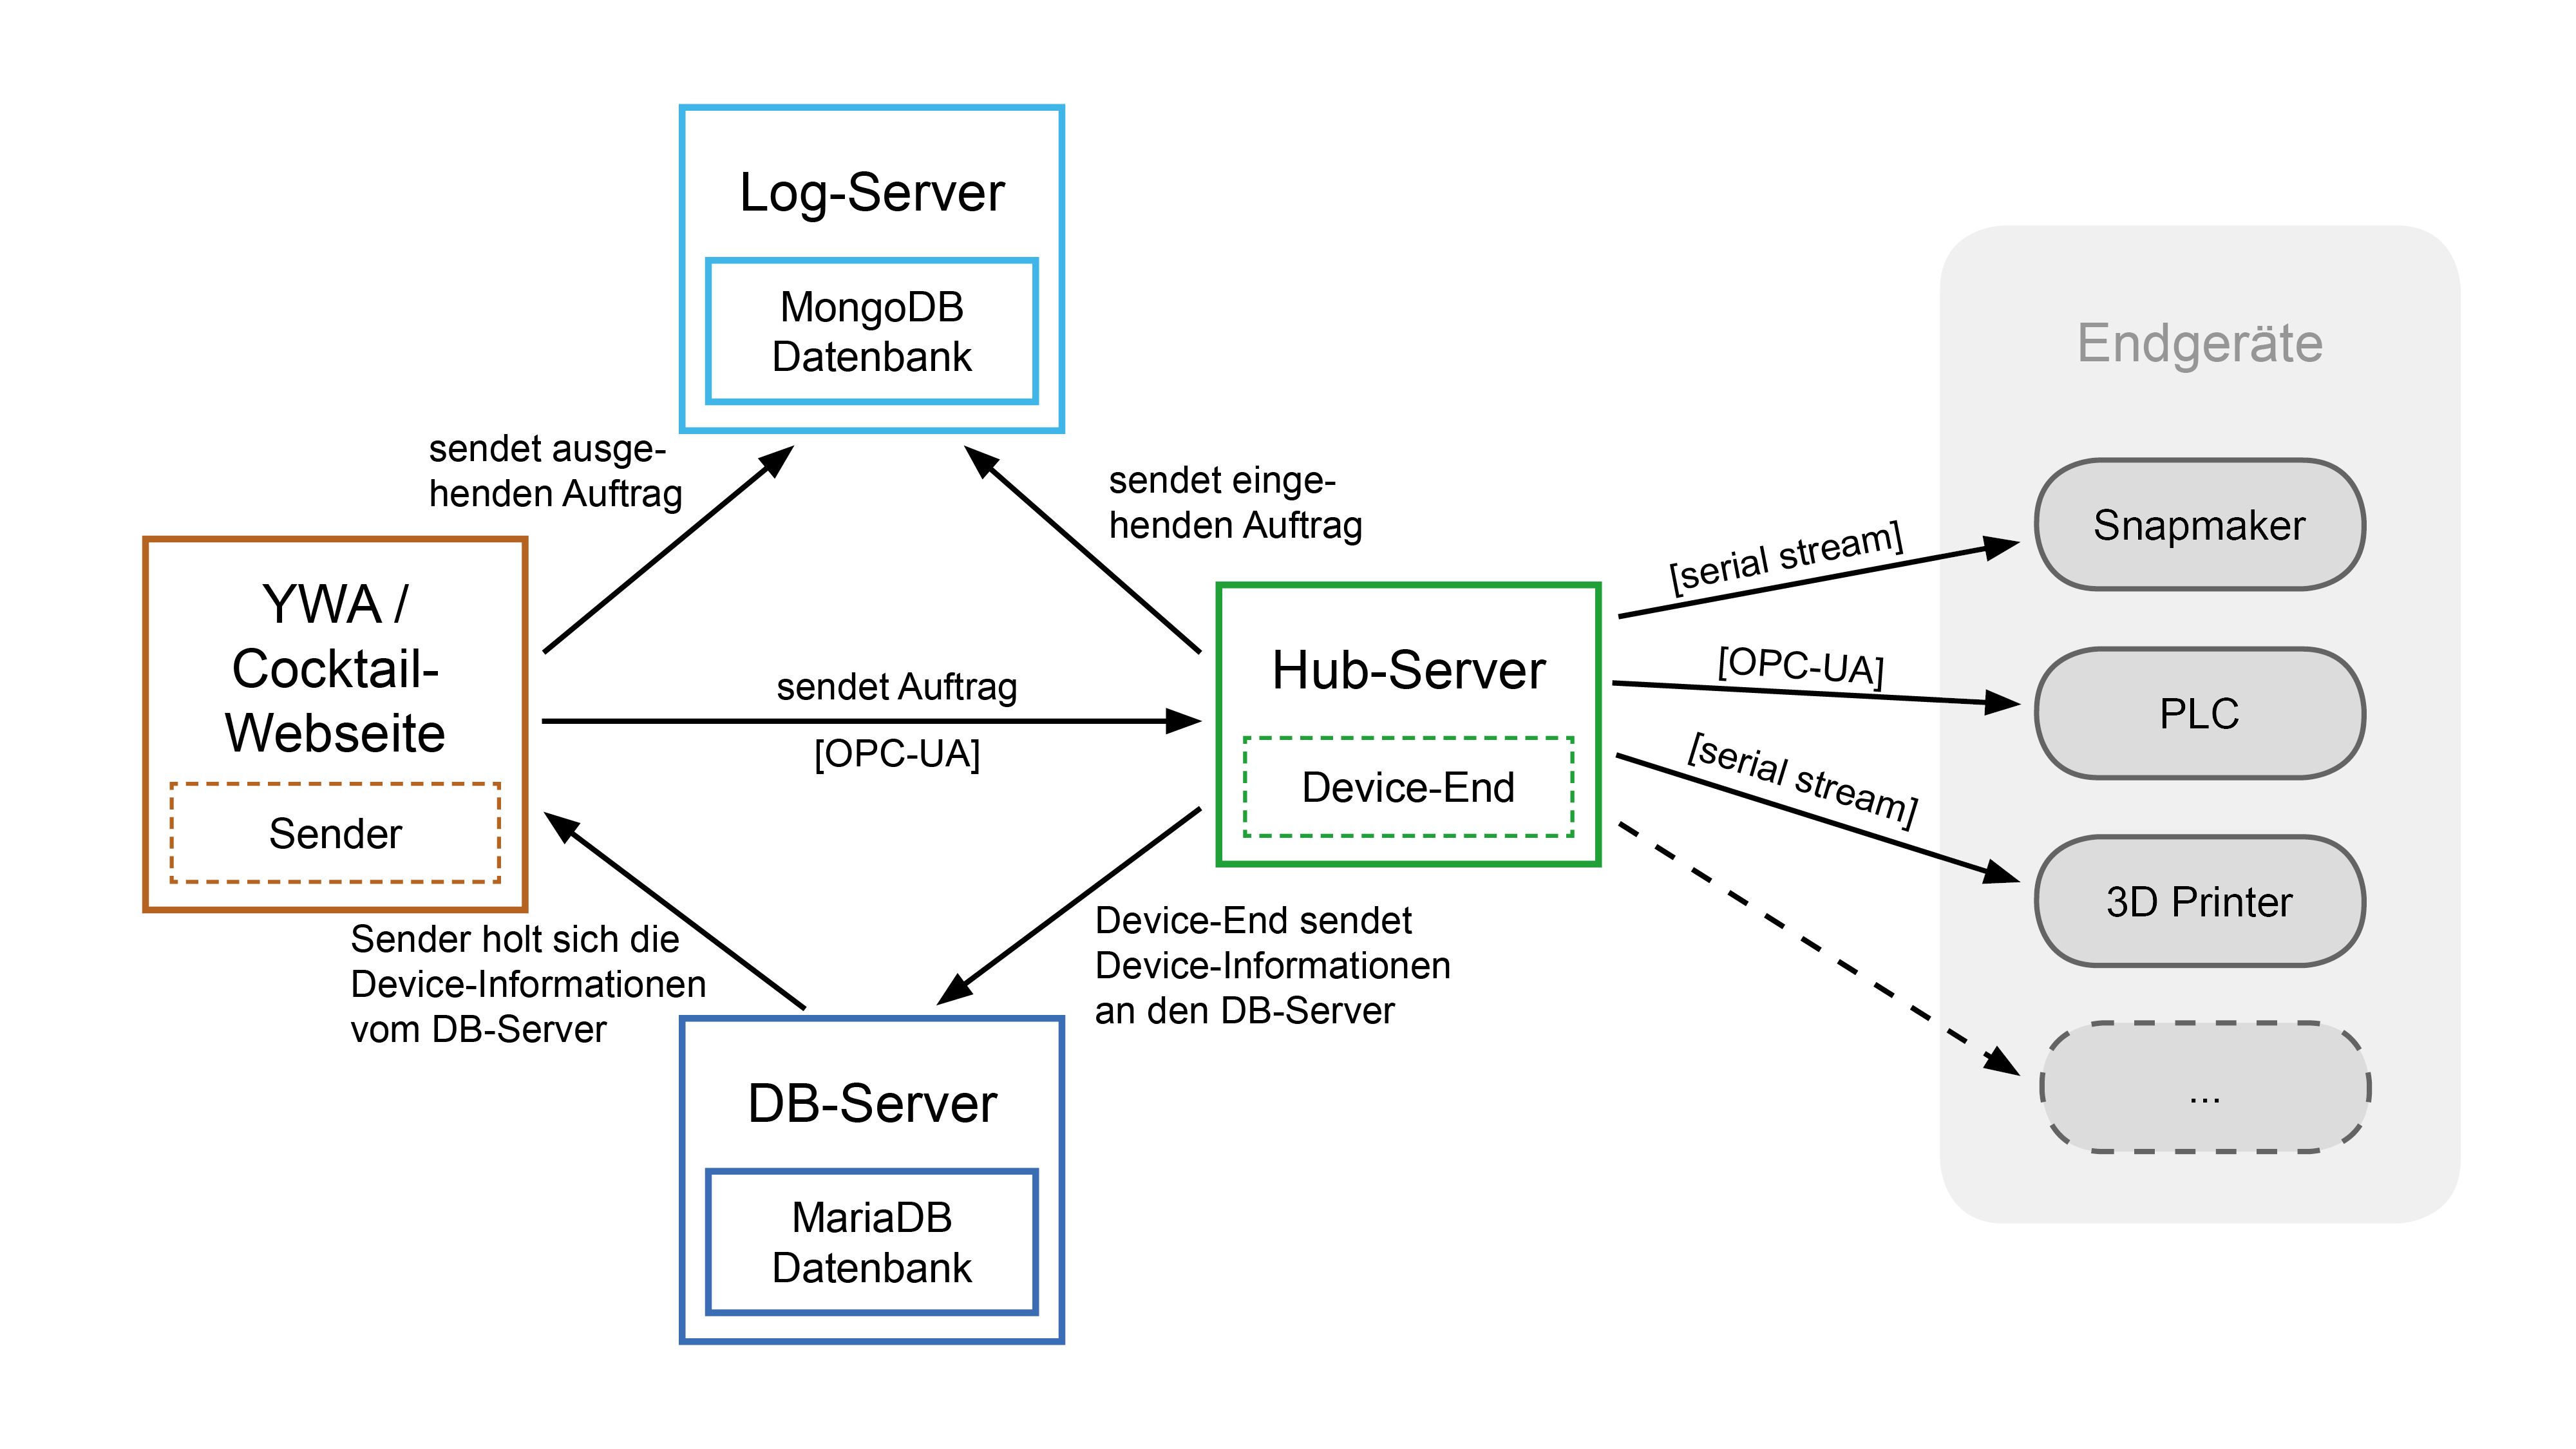
\includegraphics[width=1.0\textwidth]{images/04/BP_Project_Overview.png}
    \caption{Kommunikations-Infrastruktur der OPC Factory [\cite{bp}]}
    \label{fig:OPCFactoryInfrastruktur}
\end{figure}

Einen Unterschied zu der in diesem Kapitel \ref{cha:prozessplanungUndProzesssteuerung} behandelten Applikation ist, dass bei der OPC Factory nur vordefinierte Aufträge ausgewählt und abgeschickt werden können. Um dies so zu erweitern, dass auch individuelle Aufträge erstellt werden können, muss ein großer Fokus auf einem benutzerfreundlichen und dennoch mächtigen Interface liegen.
